

\documentclass[12pt]{article}
\usepackage[T1]{fontenc}
\usepackage[utf8]{inputenc}
\usepackage{amsmath}
\usepackage{microtype}
\usepackage{listings}
\setlength{\parindent}{0pt}
\usepackage{fancyvrb}
\usepackage{enumerate}
\usepackage{array}
\usepackage[breaklinks=true,linktocpage,hidelinks]{hyperref}
\usepackage[letterpaper]{geometry}
\usepackage{url}
\usepackage{graphicx}
\usepackage{fullpage}
\usepackage{caption}
\captionsetup{labelfont={bf,small,sf}, textfont={small, sf}}
\usepackage[sc]{mathpazo}

\usepackage{pgfplots}
\usepackage{pgfplotstable}
\usepackage{tikz}

\usepackage{fancyhdr}
\usepackage{fancybox}
\usepackage{multicol}
\usepackage{xcolor}
\usepackage{adjustbox}
\usepackage{wrapfig}



\pgfplotsset{compat=newest}
\usetikzlibrary{shapes,backgrounds,arrows}
\usepgfplotslibrary{external} 

\definecolor{brewcol1}{RGB}{166,206,227}
\definecolor{brewcol2}{RGB}{31,120,180}
\definecolor{brewcol3}{RGB}{178,223,138}
\definecolor{brewcol4}{RGB}{51,160,44}
\definecolor{brewcol5}{RGB}{251,154,153}
\definecolor{brewcol6}{RGB}{227,26,28}
\definecolor{brewcol7}{RGB}{237,179,1}
\definecolor{brewcol8}{RGB}{202,178,214}
\definecolor{brewcol9}{RGB}{206,27,1}

\definecolor{brewforest1}{RGB}{65,171,93}
\definecolor{brewforest2}{RGB}{161,217,155}
\definecolor{brewforest3}{RGB}{49,163,84}

\geometry{hmargin=1.87cm, vmargin=1.87cm}
\bibliographystyle{siam}

\DeclareTextFontCommand{\helvetica}{\fontfamily{phv}\selectfont\small}


\begin{document}

\clearpage\thispagestyle{empty}
\begin{center}
\textbf{Difficult transition for sugar maple in Boreal forest under climate change? \\
Impact of alternative stable states on Sugar maple migration.}
\vskip 2em
Research proposal
\vskip 1em
Master in Wildlife management
\vfill
By
\vfill
Steve Vissault 
\vfill 
For
\vfill
\textbf{Richard Cloutier}, Pr.\\
Director of the program committee
\vskip 2em
\textbf{Dominique Arsenault}, Pr.\\
President of the jury
\vskip 2em
\textbf{Matt Talluto}, PhD\\
Research Co-director
\vskip 2em
\textbf{Dominique Gravel}, Pr.\\
Research Director
\vfill
\vfill
Université du Québec à Rimouski\\
\today

\end{center}

\newpage
\setcounter{page}{1}

\section{Introduction}

\textbf{Context.}  The boreal region is warming twice as fast as the global
average and  this will inevitably alter the species composition in boreal
forests \cite{Scheffer2012,Hughes2000}.  Sugar maple (\textit{Acer saccharum})
is one of the species expected to migrate northward towards the northern limit
of the temperate forest \cite{McKENNEY2007,Goldblum2005}. Predicting shifts in
the range of sugar maple under climate change is an important challenge
because this species is highly desirable by hardwood and maple syrup
producers, two large economic sectors in Quebec. Indeed, sugar maple is a
widespread and abundant tree in north-eastern North America and is one of the
most representative species of northern temperate forests
\cite{Graignic2013,Messaoud2007,Kellman2004,Barras1998}. The expected
northward migration of sugar maple and its vegetal community during climate
change will increase the ecotone between the boreal and temperate forest of
Quebec. Nevertheless, the expansion of species distribution occuring in Nordic
temperate forest could be difficult to predict because microclimatic
conditions found in boreal forests are different from those present in
temperate forest. Colder temperatures from shading and excess soil moisture
due to snow melt cause litter to be more acidic and fibrous during the spring
in boreal forests . Therefore, even if the regional climate conditions are
favorable \cite{Kellman2004}, the microbiota and microclimatic conditions
found in the boreal forest could affect the establishment of sugar maple
\cite{Kellman2004,Moore2008,DeFrenne2013,Barras1998}. In this case, the sugar
maple could be unable to migrate in boreal forests as a result of negative
soil feedback. This phenomenon could increase the tension between the boreal
and temperate forest and generate abrupt changes in the community composition
(\textbf{$H_0$}).\\

\textbf{Objectives.} This project aims to develop a state
and transition model (STM) of the boreal and temperate forests in order to
investigate shifts in the distribution of sugar maple into the boreal-
temperate forest dynamical system.To assess this main objective, I will (1)
create a  model of the transition between the temperate and the boreal forest;
(2) investigate the spatial structure and presence of alternative stable states in the
transitional zone; and finally (3) run simulations based on different climate
change scenarios.  In order to define the context of this study, the first
section of this project proposal is a review subdivided into two parts. The
first part presents the theoretical context on alternative stable states and
abrupt changes in ecosystems functioning. The second part of this review
focuses on the sugar maple , its community and co-existing species in the
temperate forest and thus explain why alternative stable states is a relevant
framework to study the dynamic of the boreal-temperate forests ecotone.  The
second section of this document describes the model and the methodology
employed to assess the objectives. To conclude, the last part presents the
general timeline associated with this project.

%%% Question from hedvig: What is the relationship between the temperatre forest and the sugar maple?

\section{Review} 

\begin{figure}[t]
	\begin{center}
	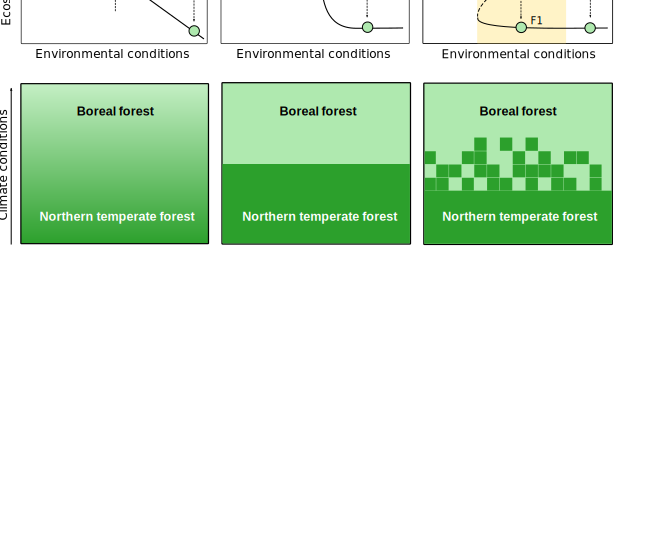
\includegraphics[width=0.8\textwidth]{fig/states.pdf}
	\end{center}
	\caption{Schematic representation of different ways in which the equilibrium
	states from forest-forest system can vary with conditions such as temperature, precipitation
	or soil moisture. Three differents kinds of respond are presented,
	\textbf{(A)} gradual, \textbf{(B)} basic fold, \textbf{(C}) catastrophic fold.
	The first panels line is a conceptualization of a transitional landscape
	between the boreal (light green) and the nordic temperate forests (dark
	green). The second panels line presents the stable states rise by the forest
	given a specific environnemental condition. Each arrows in graphs indicate the
	point toward the system moves if it's not at the equilibrium. Every point on
	the plain line could be a stable state encounter by the boreal-temperate
	forests system, excepted for the dashed line (in yellow highlight). This zone,
	called hysteresis, are particulary unstable and little fluctuations in
	environnement conditions give rise to a contrasted state representing an
	alternative stable states. ($F_1$ or $F_2$).}
	\label{fig1}
\end{figure}

% Comments from Hedvig on theoretical framework section: This first part of the review is nice and well explained, but isn’t the theoretical framework, it’s about the forest… But I think it’s better to describe ASS while you talk about forests, to make it clear. Just change the title to ‘ASS in forests’ or something

\textbf{Theorerical framework.}  Many ecotone studies and modeling efforts on
transition between forest to non-forests (e. g. Boreal - Tundra)
\cite{Scheffer2012,Scheffer2001,Hirota2011} but little attention has been
given to evaluate the transitional dynamics of forest- forest ecotones
\cite{Goldblum2010,Graignic2013}. At large scale, transition between  the
temperate and boreal forests can be approach as a dynamic system where each
forest biomes is a stable state. The presence of different states at a
location or a time depends on environmental conditions (e. g. soil,
temperature) encountered by the system. When small environmental fluctuations
occur, most dynamical system responds almost linearly with no threshold to
drastic changes in the state of the ecosystem ( Figure \ref{fig1} .A)
\cite{Scheffer2001,Scheffer2009}. In this case, only one equilibrium can be
observed given a specific environmental condition
\cite{Scheffer2001,Scheffer2009,scheffer2009critical}.  When the soil moisture
increase slowly, the new condition obtained might cause favorable conditions
to a new species, but this species establishment doesn't change the entire
community therefore the ecosystem functionning. Another kind of response
occurs more frequently in nature.  Natural systems are insensitive to
environmental conditions over certain ranges but respond strongly when a
threshold is reached (Figure \ref{fig1} .B) \cite{scheffer2009critical}. For
example, tree mortality can increase sharply when a toxin is added to the
environment. \cite{scheffer2009critical}. In this case, the response curve of
the natural systeme is not linear and lightly folded and a small change can
drive the sytem to a treshold and lead to major changes. As an example, small
changes in the initial conditions can transform abruptly the species community
composition and lead to a strong spatial division as representing in figure
\ref{fig1} .C (Upper panel). In an other hand, respond curve can be folded
backwards and the same threshold can conduct the system into catastrophic
changes (Figure \ref{fig1} .C).  When the system approach a tipping point on
the folded upper branch, the system cannot pass smootly to the lower branch.
Small forcing on initial condition of the state $F_1$ transfer immediatly the
system into a contrasted state $F_2$ (Figure \ref{fig1} .C). This point is
called \textit{Bifurcation point} and small forcing on those critical states
can drive the system into backward or forward shifts, increasing catastrophic
events. In this situation, the system present alternative stable states who
certain range of environnemental conditions. This range correspond to the
hysteresis zone and can be seen as an intermixed patches in the forest-forest
ecotone landscape like shown across the sub-figure \ref{fig1} .C (upper part).
\\

 %% Transition sentence

\textbf{Natural system.} In the boreal-temperate forest ecotone, there is no
distinct boundary and a broad transition zone exists composed of mixed stands
of coniferous-deciduous species \cite{Goldblum2010}. In this ecotone, a macromosaic landscape can be observed with pure stands of deciduous trees on favorable sites and pure coniferous stands on less favorable sites
\cite{Goldblum2010}. Knowing this, the alternative stable states is a relevant
framework to study this ecotone dynamic because the soil seems to have a
negative feedback on the temperate forest establishment. This phenomenon need
to be investigate has a main attractor in alternative stable states
\cite{Kellman2004,Moore2008,DeFrenne2013,Barras1998}. 


% L'écotone entre la forêt boréal et la forêt tempérée
% nordique. La répartition des espèces caractéristiques de ces milieux ne sui
% pas un gradient climatique mais concorde avec un gradient lié à la texture et
% à la composition du sol. Plusieurs espèces clés représentent fortement les
% communautés végatles rattachés à ces biomes. Ces espèces germent sur des
% conditions de sols contrastés contribuant à maintenir la présence


% We used maple sugar basa areal in function of black
% spruce, white spruce and balsam fir basal area to compute the relative
% abundance of sugar maple. Given the above statements, we used mainly two
% climatic variables (annual mean temperature and annual precipitation) to
% identify the alternative stable states present in the boreal-temperate
% ecotone. The relationship was performed on climatic variables and sugar maple
% relative abundance using kernel density plot function. We obtained the
% probability of observed a sample plot as function of sugar maple relative
% abundance and mean annual temperature (Figure \ref{fig1}). In both case,
% alternative stable states are presents whereas the function graphed has a
% bimodal distribution. At low precipitation or temperature conditions, the
% probability of observing a parcel sampled without sugar maple is higher than
% intermediate climatic conditions where the multimodal distribution appear. The
% density function suggest the presence of alternative stabe states  in response
% of intermediate climatic conditions: one state wherein sugar maple dominates
% and an another in which sugar maple is absent. \\
\section{Methods}   

%% Transition sentence

\begin{wrapfigure}{L}{0.45\textwidth}         
	
	\begin{figure}[!ht]
\begin{center}
	
				\tikzstyle{noeud}=[circle,
				                  thick,
				                  minimum size = 1.5cm,
				                  inner sep =5pt,
				                  draw=brewforest3,
				                  fill=brewforest1]
				\tikzstyle{noeud2}=[circle,
				                  thick,
				                  minimum size = 1.5cm,
				                  inner sep =5pt,
				                  draw=brewforest3,
				                  fill=brewforest2]
				\tikzstyle{noeud3}=[circle,
				                  thick,
				                  minimum size = 1.5cm,
				                  inner sep =5pt,
				                  draw=brewforest3,
				                  fill=brewforest3]
	
				\begin{tikzpicture}[->,>=stealth',auto,scale=0.8]
				      \node [circle,noeud2] (M) at (0,0) {\textbf{M}};
				      \node [circle,noeud2]  (C) at (-5,5) {\textbf{C}};
				      \node [circle,noeud2] (D) at (5,5) {\textbf{D}};
				      \node [circle,noeud2] (T) at (0,10) {\textbf{T}};
	
						\draw[thick,-latex] (M) to[bend right=10] node[above,sloped] {$S_C$} (C);
						\draw[thick,-latex] (C) to[bend right=10] node[below,sloped] {$\beta_d \cdot (C+M)$} (M);
	
						\draw[thick,-latex] (D) to[bend right=10] node[above,sloped] {$\beta_c \cdot (D+M)$} (M);
						\draw[thick,-latex] (M) to[bend right=10] node[below,sloped] {$S_D$} (D);
	
						\draw[thick,-latex] (D) to[bend right=10] node[above,sloped] {$e$} (T);
						\draw[thick,-latex] (T) to[bend right=10] node[below,sloped] {$P_D$} (D);
	
						\draw[thick,-latex] (T) to[bend right=10] node[above,sloped] {$P_C$} (C);
						\draw[thick,-latex] (C) to[bend right=10] node[below,sloped] {$e$} (T);
	
						\draw[thick,-latex,transform canvas={xshift=0.8ex}] (T) to node[above,sloped,rotate=90,transform canvas={xshift=5ex}] {$P_D \cdot P_C$} (M);
						\draw[thick,-latex,transform canvas={xshift=-0.8ex}] (M) to node[above,sloped,rotate=-90,transform canvas={xshift=-3ex}] {$e$} (T);
				\end{tikzpicture}
	
			\caption{Conceptual transition model between forest stands deciduous ($D$), mixte ($M$) and coniferious ($C$). $E$ corresponds to a transitionnal state where a perturbation are occurred with a frequence of $e$. Parameters $\beta$ and $S$ are referred as the colonisation and the succession rates respectively. We defined the recovery rates ($P_C$ et $P_D$) as $P_C = \alpha_C \cdot (M+C) \cdot [1- \alpha_D \cdot (D +M)]$ and $P_D = \alpha_D \cdot (D+M) \cdot [1- \alpha_C \cdot (C +M)]$, to finaly get this equation $P_M = P_C \cdot P_D$. The parameter $\alpha$ mean the recovery rate after a patch has been disturbe.}

	\end{center}	
	\label{Model}
\end{figure}
	\caption{Conceptual transition model between forest stands deciduous ($D$),
	mixte ($M$) and coniferous ($C$). $T$ corresponds to a transitionnal state
	where a perturbation are occurred with a frequence of $e$. Parameters $\beta$
	and $S$ are referred as the colonisation and the succession rates
	respectively. We defined the recovery rates ($\phi_c$ et $\phi_d$) as $\phi_c
	= \alpha_c \cdot (M+C) \cdot [1- \alpha_d \cdot (D +M)]$ and $\phi_D =
	\alpha_d \cdot (D+M) \cdot [1- \alpha_c \cdot (C +M)]$, to finaly get this
	equation $\phi_m = \phi_c \cdot \phi_d$. The parameter $\alpha$ mean the
	recovery rate after a patch has been disturbe.}         
	\label{Model}
\end{wrapfigure}

\textbf{Models.} This state and transition model will be based on three
different forest states: \textbf{(D)} Deciduous and \textbf{(M)} Mixed patches
characterizing temperate forests, then \textbf{(C)} Coniferous patch
representing boreal forests (Figure \ref{Model}). Disturbances regime is a main
driver in those forest dynamics (e .g. Fire in boreal forest or frost in
temperate forest). When gap event occur in deciduous patch, species presents
will be replaced by shade intolerant species as aspen and white birch, well
adapted to the new shading condition. Thus post-disturbance patches has been
integrated within the model across the transitional patch \textbf{(T)} (Figure
\ref{Model}).  On long term, late-succesional species from the understory will
take up giving a new state (C, D or M). All states can change to another state
except the direct transition between a deciduous and coniferous stands which
doesn't occur in natural systems. Simulations of this model aims to assess the
transition rate between each state in the overall landscape and identify if
deciduous and coniferous patches are present as alternative stable states. When
a coniferous patch $C$ has been disturbed with a rate $e$, this can be recovered
to another state following $\phi_c$. This term is taking in account a specific
patch recovery rate ($\alpha_{c}$), the availability of coniferous species
($M+C$) and the proportion of paths unconverted into a deciduous state ($1-
\alpha_d \cdot (D +M)$). In making the assumption that perturbation rate is
similar between states, dynamic of a patch $T$ can be formally describe by these
differential equations: $\frac{\delta T}{\delta t} = e \cdot (C+M+D) - T \cdot
(\phi_d + \phi_c + \phi_m)$. If a patch $C$ is undisturbed, deciduous species
$(D+M)$ can spread over the patch with a colonisation rate $\beta_d$ giving a
new mixed patch. A mixed stand $M$ might turn into a coniferous stand with a
sucession rate $S_c$.  We can also summarize the coniferous dynamic by this
differential equation: $\frac{\delta C}{\delta t} = \phi_C \cdot T + S_c \cdot M
- \alpha_d \cdot (D+M)\cdot C - e \cdot C$. At this stage of this project, the
model is spatially implicit and assume that all space is occupied by one state,
so that the proportions of land cover occupied by all types of patch sum to 1.
\\

\textbf{Paramerization.} The parameterization of this model will be conducted
on the QUICC-FOR database containing large permanent sample plots surveys.
Those data are provided by several forest offices and cover multiple canadian
provinces ($\pm16 000$ plots) and states ($\pm50 000$ plots). These
inventories started since the 1970s and include all stems measurements and
forest stand informations relative to a specific plot location and year. The
basal area will be compute to provide a measure of relative growth by species
present and plots. Each plot will be classified into the four different states
following their percent of  deciduous and coniferious cover.   

To include the climate, each model parameters will be calibrate as a
function of probability based on climatic conditions. Climate is a main driver
in the distribution of those biomes, but their dynamics are also strongly related
to their own disturbance regimes (i. e. Fire in boreal forest, frost in
temperate forest) \cite{Goldblum2010}. % Quelles variables climatique sont intégré ? \\

\textbf{Simulation.} This model will be incorporated in a spatially explicit cellular automaton or lattice in
order to evaluate the velocity of the transition into differents patches and differents
climate change scenario.

% - Temps discrets
% - Cellulaire automate\\

\textbf{Validation.} 
% - Matrice de confusion sur la classification des patchs (M,D,C,T)
% - Matrice de confusion (TSS) et AUC sur un jeux de données indépendants 
% - Spatialement explicit à l'aide de l'automate cellulaire.


\newpage
\bibliography{/home/steve/Dropbox/Bibtex/Devis}
\end{document}

%%%%%%%%%%%%%%%%%%%%%%%%%%%%%%%%%%%%%%%% 
%%% Extra

%We will assume that all space is occupied by one state, so that the proportions of land cover occupied by all types of patch sum to 1.

%\frac{\delta C}{\delta t} = \alpha_C \cdot (C+M) \cdot (1-\alpha_D \cdot (D+M)) \cdot (1-C-D-M) + S_C \cdot M - \%beta_D \cdot (D+M) \cdot C - e \cdot C%
%\frac{\delta D}{\delta t} = \alpha_D \cdot (D+M) \cdot (1-\alpha_C \cdot (C+M)) \cdot (1-C-D-M) + S_D \cdot M - %\%beta_C \cdot (C+M) \cdot D - e \cdot D
%\frac{\delta M}{\delta t} = \alpha_C \cdot (C+M) \cdot \alpha_D \cdot (D+M) \cdot (1-C-D-M) + \beta_C \cdot (C+M) + \beta_D \cdot (D+M) - S_C \cdot M - S_D \cdot M - e \cdot M

% \begin{figure}[!ht]
% 	\centering
% 	\begin{minipage}{0.45\linewidth}
% 		
	\begin{figure}[!ht]
\begin{center}
	
				\tikzstyle{noeud}=[circle,
				                  thick,
				                  minimum size = 1.5cm,
				                  inner sep =5pt,
				                  draw=brewforest3,
				                  fill=brewforest1]
				\tikzstyle{noeud2}=[circle,
				                  thick,
				                  minimum size = 1.5cm,
				                  inner sep =5pt,
				                  draw=brewforest3,
				                  fill=brewforest2]
				\tikzstyle{noeud3}=[circle,
				                  thick,
				                  minimum size = 1.5cm,
				                  inner sep =5pt,
				                  draw=brewforest3,
				                  fill=brewforest3]
	
				\begin{tikzpicture}[->,>=stealth',auto,scale=0.8]
				      \node [circle,noeud2] (M) at (0,0) {\textbf{M}};
				      \node [circle,noeud2]  (C) at (-5,5) {\textbf{C}};
				      \node [circle,noeud2] (D) at (5,5) {\textbf{D}};
				      \node [circle,noeud2] (T) at (0,10) {\textbf{T}};
	
						\draw[thick,-latex] (M) to[bend right=10] node[above,sloped] {$S_C$} (C);
						\draw[thick,-latex] (C) to[bend right=10] node[below,sloped] {$\beta_d \cdot (C+M)$} (M);
	
						\draw[thick,-latex] (D) to[bend right=10] node[above,sloped] {$\beta_c \cdot (D+M)$} (M);
						\draw[thick,-latex] (M) to[bend right=10] node[below,sloped] {$S_D$} (D);
	
						\draw[thick,-latex] (D) to[bend right=10] node[above,sloped] {$e$} (T);
						\draw[thick,-latex] (T) to[bend right=10] node[below,sloped] {$P_D$} (D);
	
						\draw[thick,-latex] (T) to[bend right=10] node[above,sloped] {$P_C$} (C);
						\draw[thick,-latex] (C) to[bend right=10] node[below,sloped] {$e$} (T);
	
						\draw[thick,-latex,transform canvas={xshift=0.8ex}] (T) to node[above,sloped,rotate=90,transform canvas={xshift=5ex}] {$P_D \cdot P_C$} (M);
						\draw[thick,-latex,transform canvas={xshift=-0.8ex}] (M) to node[above,sloped,rotate=-90,transform canvas={xshift=-3ex}] {$e$} (T);
				\end{tikzpicture}
	
			\caption{Conceptual transition model between forest stands deciduous ($D$), mixte ($M$) and coniferious ($C$). $E$ corresponds to a transitionnal state where a perturbation are occurred with a frequence of $e$. Parameters $\beta$ and $S$ are referred as the colonisation and the succession rates respectively. We defined the recovery rates ($P_C$ et $P_D$) as $P_C = \alpha_C \cdot (M+C) \cdot [1- \alpha_D \cdot (D +M)]$ and $P_D = \alpha_D \cdot (D+M) \cdot [1- \alpha_C \cdot (C +M)]$, to finaly get this equation $P_M = P_C \cdot P_D$. The parameter $\alpha$ mean the recovery rate after a patch has been disturbe.}

	\end{center}	
	\label{Model}
\end{figure}
% 	\end{minipage}
% 	\begin{minipage}[t]{1\linewidth}
% \small{\begin{equation}
% 	 	\frac{\delta T}{\delta t} = e \cdot (C+M+D) -  T \cdot (\phi_D + \phi_C + \phi_M \\
% \end{equation}
% \begin{equation}
% 		\frac{\delta M}{\delta t} = \phi_M\cdot T +  \beta_C \cdot (C+M)\cdot D + \beta_D\cdot (D+M)\cdot C - S_C\cdot M -S_D\cdot M - e\cdot M \\
% \end{equation}
% \begin{equation}
% 		\frac{\delta C}{\delta t} = \phi_C \cdot T + S_C\cdot M - D\cdot (D+M)\cdot C - e \cdot C \\
% \end{equation}
% \begin{equation}
% 		\frac{\delta D}{\delta t} = \phi_D \cdot T + S_D \cdot M - \beta_C \cdot (C+M) \cdot D - e \cdot D
% \end{equation}}
% 	\end{minipage}
